% From https://tex.stackexchange.com/questions/462984/fancy-vertical-timeline

\documentclass[tikz, margin=3.141592mm]{standalone}
\usetikzlibrary{arrows.meta,
                chains,
                positioning}

\begin{document}
    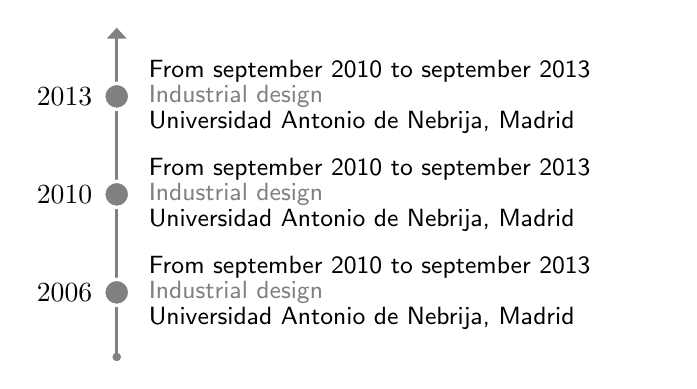
\begin{tikzpicture}[
node distance = 1mm and 3mm,
  start chain = A going below,
   dot/.style = {circle, draw=white, very thick, fill=gray,
                 minimum size=3mm},
   box/.style = {rectangle, text width=62mm,
                 inner xsep=4mm, inner ysep=1mm,
                 font=\sffamily\small\linespread{0.84}\selectfont,
                 on chain},
                        ]
    \begin{scope}[every node/.append style={box}]
\node { From september 2010 to september 2013   \\      % A-1
        \textcolor{gray}{Industrial design}     \\
        Universidad Antonio de Nebrija, Madrid} ;
\node { From september 2010 to september 2013   \\
        \textcolor{gray}{Industrial design}     \\
        Universidad Antonio de Nebrija, Madrid} ;
\node { From september 2010 to september 2013   \\      % A-3
        \textcolor{gray}{Industrial design}     \\
        Universidad Antonio de Nebrija, Madrid} ;
    \end{scope}
\draw[very thick, gray, {Triangle[length=4pt)]}-{Circle[length=3pt]},
      shorten <=-3mm, shorten >=-3mm]           % <--- here is adjusted additional arrow's 
    (A-1.north west) -- (A-3.south west);
\foreach \i [ count=\j] in {2013,2010,2006}
    \node[dot,label=left:\i] at (A-\j.west) {};
    \end{tikzpicture}
\end{document}